\section{Introduction}
\label{sec:introduction}
The following technical documentation will give further information for the implementation of the \textit{Internet Praktikum} from the group \texttt{HOTEL-Square}. The \textit{Internet Praktikum} aims at getting in touch with current web technologies, which "are becoming the basic building blocks of the next generation of Internet services"\footnote{\url{https://www.tk.informatik.tu-darmstadt.de/de/teaching/sommersemester-2017/internet-praktikum-tk-p4/}, 03.07.2017}. Therefore, state-of-the-art protocols and technologies are used to implement a specific task in a web based context.

\subsection{Task}
\label{subsec:task}
The task of the \textit{Internet Praktikum} in summer term 2017 is to reimplement a clone of the \textit{Foursquare Android} app. The task includes a well defined extend of compulsory features, which the app should support. There is the possibility of extending this compulsory feature list by some bonus features. 

In general, the task of the project includes the implementation of a well defined architecture, which comprises a development task for an \textit{Android} app (frontend) and a development task including a server in \textit{NodeJS} (backend). The backend should include a \textit{NoSQL} database and is allowed to query some third-party API-services. In opposite, the frontend is limited to communicate with the \textit{NodeJS}-server via some well-defined API. 
\newline\newline
The compulsory features of the app are:
\begin{itemize}
	\item User management:
	\begin{itemize}
		\item Create new account
		\item Login
		\item Delete account
		\item Reset password
	\end{itemize}
	\item Venue data:
	\begin{itemize}
		\item Pull venue data from the backend
	\end{itemize}
	\item Possible User Actions:
	\begin{itemize}
		\item Venue Search (at current location and in other location)
		\item Venue Search via text input and via predefined categories
		\item Search results must be displayed in a list and on a map
	\end{itemize}
	\item Venue view 
	\begin{itemize}
		\item Venue overview page showing photos and important information about the venue
		\item Look at photos that where uploaded to the venue in a photo albu with swiping
		\item Add comments with text and photos, like/dislike them and read other's comments
		\item Check into venues to show you where there
		\item Rate the venues
		\item Show the current top visitors of a venue
	\end{itemize}	
	\item Map
	\begin{itemize}
		\item Show venues on the map, click on them to get to the venue overview
		\item Show the user's location on the map
		\item Show the user's friends location on the map
	\end{itemize}
	\item User profile
	\begin{itemize}
		\item Profile view
		\item Profile fields containing the user name, real name, age and city
		\item Picture
		\item Profile editing for the user's own profile
	\end{itemize}
	\item Friends
	\begin{itemize}
		\item Find friends by name/user name, through comments on venues or on the map
		\item Friend list showing the user's friends with links to their profile
		\item Chat/messaging with the user's friends
	\end{itemize}
	\item Venue Gamification
	\begin{itemize}
		\item User with the must "checkins" in a venue is the "king"
	\end{itemize}
\end{itemize}

Proposed bonus features for the app are:
\begin{itemize}
	\item User management:
	\begin{itemize}
		\item Facebook/other login
		\item E-Mail confirmation
	\end{itemize}
	\item Search Results:
	\begin{itemize}
		\item must be filterable
	\end{itemize}
	\item Map
	\begin{itemize}
		\item Live update of the user's friends location
	\end{itemize}
	\item Friends
	\begin{itemize}
		\item Privacy measures
	\end{itemize}
	\item Venue Gamification
	\begin{itemize}
		\item Any gamification is a bonus
	\end{itemize}
\end{itemize}

The compulsory features of the server are:
\begin{itemize}
	\item Implementation of the server in \textit{NodeJS}
	\item Usage of a \textit{NoSQL} database for storage
	\item Implementation of a \texttt{REST}-ful API for the app-calls (\texttt{CRUD} for comments, ratings, pictures and ALL possible acitons)
	\item Hosting of the server
	\item Pull venue data from \textit{Google} (or similar service)	
\end{itemize}

Besides implementing all of the above mentioned compulsory features, the following table lists all bonus features, which were further on implemented:

\begin{table}[htbp]
	\centering
	\label{tab:bonus_features}
	\begin{tabular}{c}
		General \\
		\hline\hline
		Privacy means: "incognito modus" 
		-> if applied, no one can see the user's location and vice versa \\
		\hline
		Live update of the user's friends location on the map \\
		\hline
		Filterable search results (opening hours/costs) \\
		\hline
		E-mail confirmation for registration and password reset (secured by SSL and DKIM) \\
		\hline
		\\
		\hline\hline
		Frontend \\
		\hline\hline
		two languages: Deutsch and English  \\
		\hline
		different marker colors on map depending on rating \\
		\hline
		different accuracy-strategies to optimize accuracy/battery consumption \\
		\hline
		Button to directly call the venue \\
		\hline
		Button to open the Website of a venue \\
		\hline
		Jump to the profile of your friend by clicking on his marker info window \\
		\hline
		Button to find your own Position on the map \\
		\hline
		Display the last message of a chat as a preview in the inbox.  \\
		\hline
		Highlighting of chats with unread messages in the inbox. \\
		\hline\hline
		Backend \\
		\hline\hline
		BDD/TDD -> Chai \\
		\hline
		CD -> test/static code analysis (Lint, test code coverage)/use of docker containers for deployment \\
		\hline
		use of \textit{bcrypt} library for secure password hashing \\
		\hline
		S3 filehosting with \textit{min.io} \\
		\hline
		Stateless server realized with \textit{JWT} (\textit{JSON Web Token}) \\
		\hline
		Security measures: SSL for whole API \\
	\end{tabular}
\caption{Bonus features of HOTELsquare}
\end{table}



\subsection{General Architecture}
\label{subsec:general_architecture}
To accomplish the given task of implementing a Foursquare clone the general architecture was prescribed in the project definition. As shown in fig.\ (\ref{fig:architecture}), a \textit{NodeJS} server should provide an API for the \textit{Android} app. The server itself shall work based on a \textit{NoSQL} database such as \textit{MongoDB}, which is used in the presented project. The server is allowed to fetch venue data from the \textit{Google Places API} and deliver them to the app. 

\begin{figure}[htbp]
	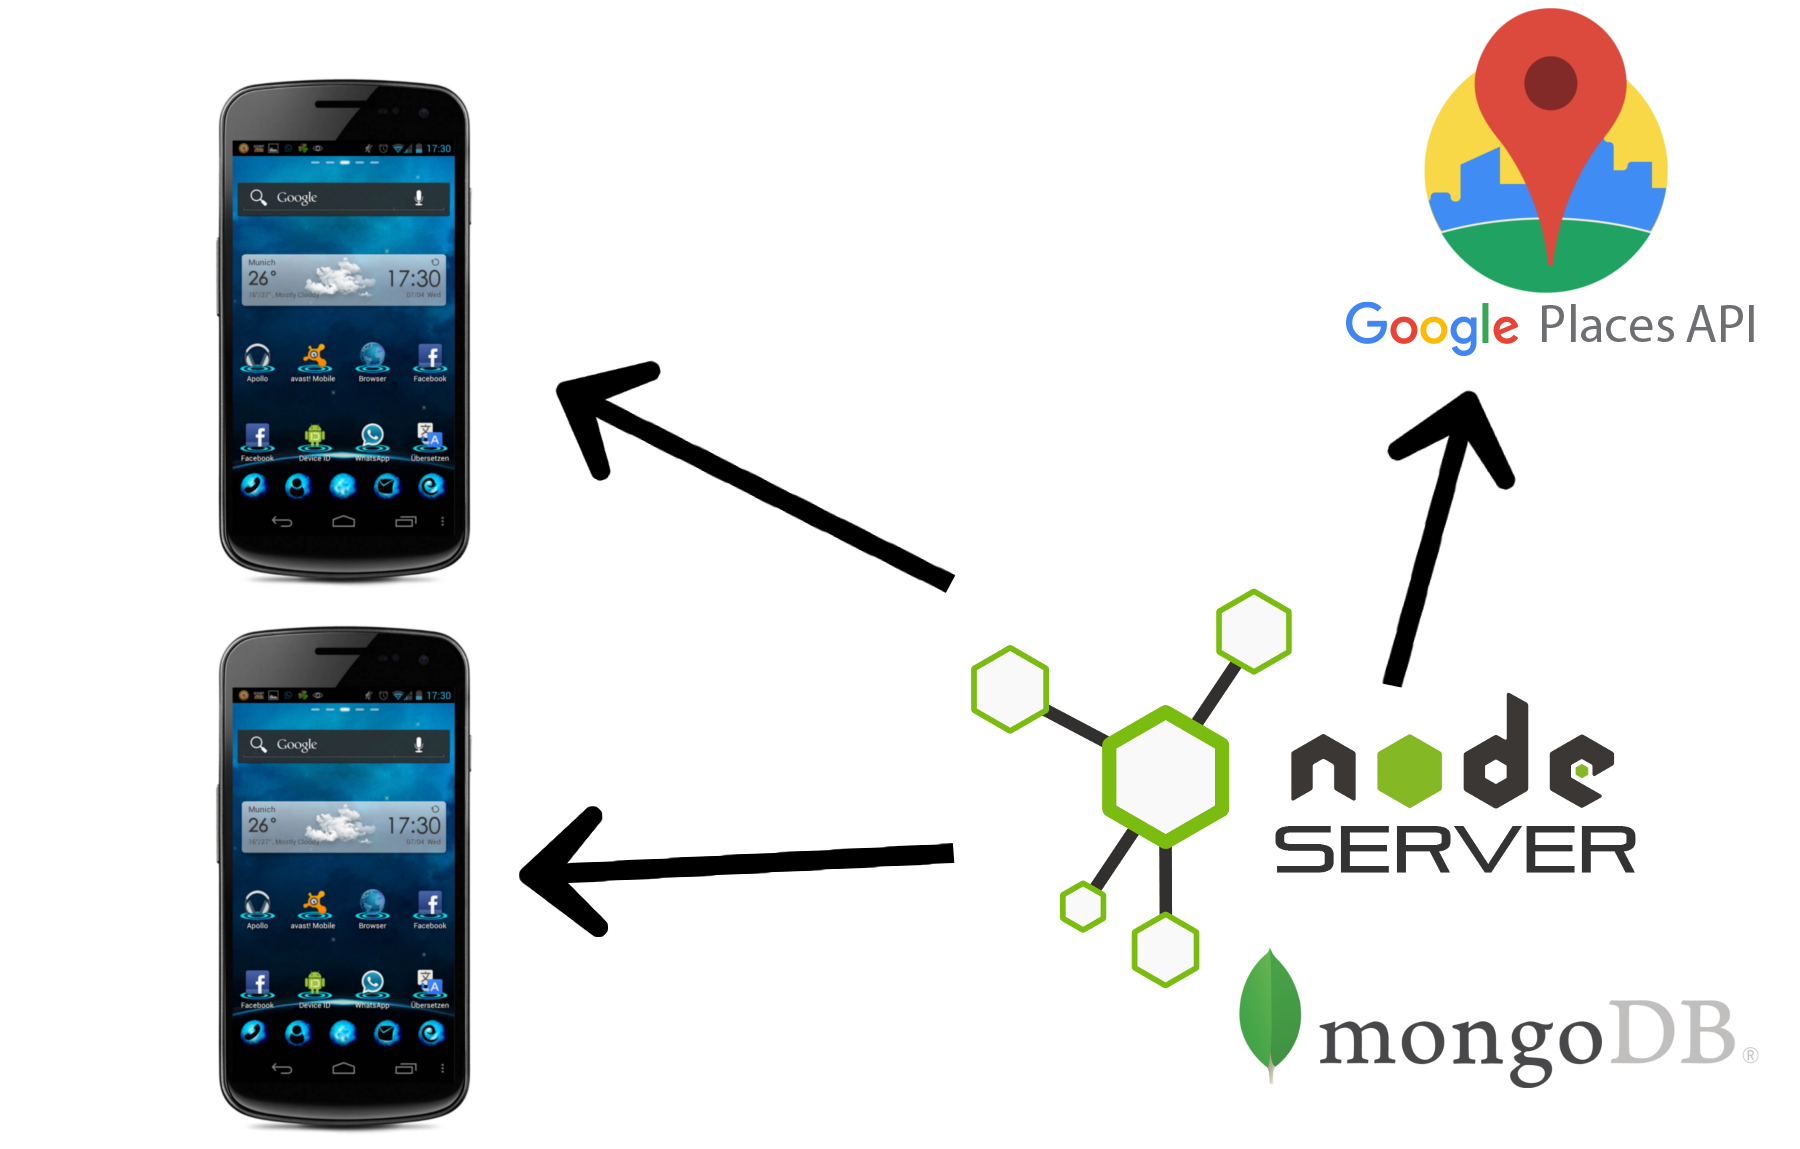
\includegraphics[width=0.8\textwidth]{images/architecture.png}
	\centering
	\caption[Project architecture]{The server written in \textit{NodeJS} with a \textit{MongoDB} database pulls venue data from \textit{google places API}. The server provides an API for the \textit{Android} app.\footnotemark}
	\label{fig:archtecture}
\end{figure} 

\footnotetext{Images taken from: \url{https://raw.githubusercontent.com/altairstudios/nodeserver/master/nodeserver-logo.png}, \url{http://www.chip.de/ii/1/5/9/3/1/1/1/6/609e955b0a179dab.jpg}, \url{https://webassets.mongodb.com/_com_assets/cms/MongoDB-Logo-5c3a7405a85675366beb3a5ec4c032348c390b3f142f5e6dddf1d78e2df5cb5c.png}, \url{http://www.ceda.cz/files/logo/google/google_2016/icon_placesapi.png}, \url{https://www.webgeoservices.com/wp-content/uploads/2017/02/Google-Places-API.jpg} (24.07.2017)}

\subsubsection{Dedicated Server}
\label{subsubsec:dedicatedserver}
To fulfil the given task, it was necessary to have access to a physical or virtual server to run the web server for the backend. We chose to use an already available dedicated server where the current status of the web server could always directly be deployed to. Under \url{https://dev.ip.stimi.ovh/}, the \texttt{REST}ful API of the web server was available also during the development stages as CD (Continuous Deployment) was the development style of choice for the backend (for more on that, see sec.\ \ref{sec:backend}). \newline
The hardware of the server is totally sufficient to handle even a medium amount of accesses to the backend services: 16GB RAM, Core™ i5-750, 2TB HDD, 100 Mbit/s network access speed.

\subsubsection{\textit{NodeJS}}
\label{subsubsec:nodejs}
\textit{NodeJS} is an asynchronous, event driven open-source, cross-platform \textit{JavaScript} runtime environment. Within \textit{NodeJS} \textit{JavaScript} code can be executed on server-side rather than embedding the scripts in the web page content and running them in the client's browser. With \textit{NodeJS} it is possible to build scalable network applications as callbacks are fired for each connection to the server which is a much more scalable than thread-based networking approaches.\footnote{\url{https://nodejs.org/en/about/}, \url{https://en.wikipedia.org/wiki/Node.js} (24.07.2017)}

\subsubsection{\textit{MongoDB}}
\label{subsubsec:mongodb}
\textit{MongoDB} is one of the leading \textit{NoSQL} databases. \textit{NoSQL} databases provide mechanisms for storing and retrieving data without following the approach of having tabular relations like in relational databases. \textit{MongoDB} is an open-source document-oriented database, which means that the data is stored in any kind of documents instead of a tabular model. In this case, user defined schemas are stored in \textit{JSON}-like files. By the use of auto-sharding, it is highly scalable and complex architectures across many data centres are possible.\footnote{\url{https://www.mongodb.com/de}, (24.07.2017)}

In this project, \textit{mongoose}, an object modelling format for \textit{MongoDB} data is used. It works like an ORM (object-relational mapping) tool making it easy to store data from an object oriented programming language into a relational database (Although \textit{MongoDB} is a \textit{NoSQL} database, \textit{mongoose} facilitates the handling a lot).  \textit{mongoose} helps to access the \textit{MongoDB} database in an object oriented manner providing simple \texttt{CRUD} methods and to create schemas for it. 

\subsubsection{\textit{Android}}
\label{subsubsec:android}
\textit{Android} is a wide-spread OS for mobile gadgets like smartphones, tablets, smartwatches, gaming consoles, cars or tv's. The open-source software is based on the \textit{Linux} kernel. On top, there are several software layers abstracting from the hardware as shown in fig.\ (\ref{fig:androidstack}). Most important for developers, the \textit{Java} API framework provides many state-of-the-art libraries for efficient high level access to most hardware features of the used gadget and a lot of predesigned software libraries for fast coding of apps based on the life cycle of the app.   

\begin{figure}[htbp]
	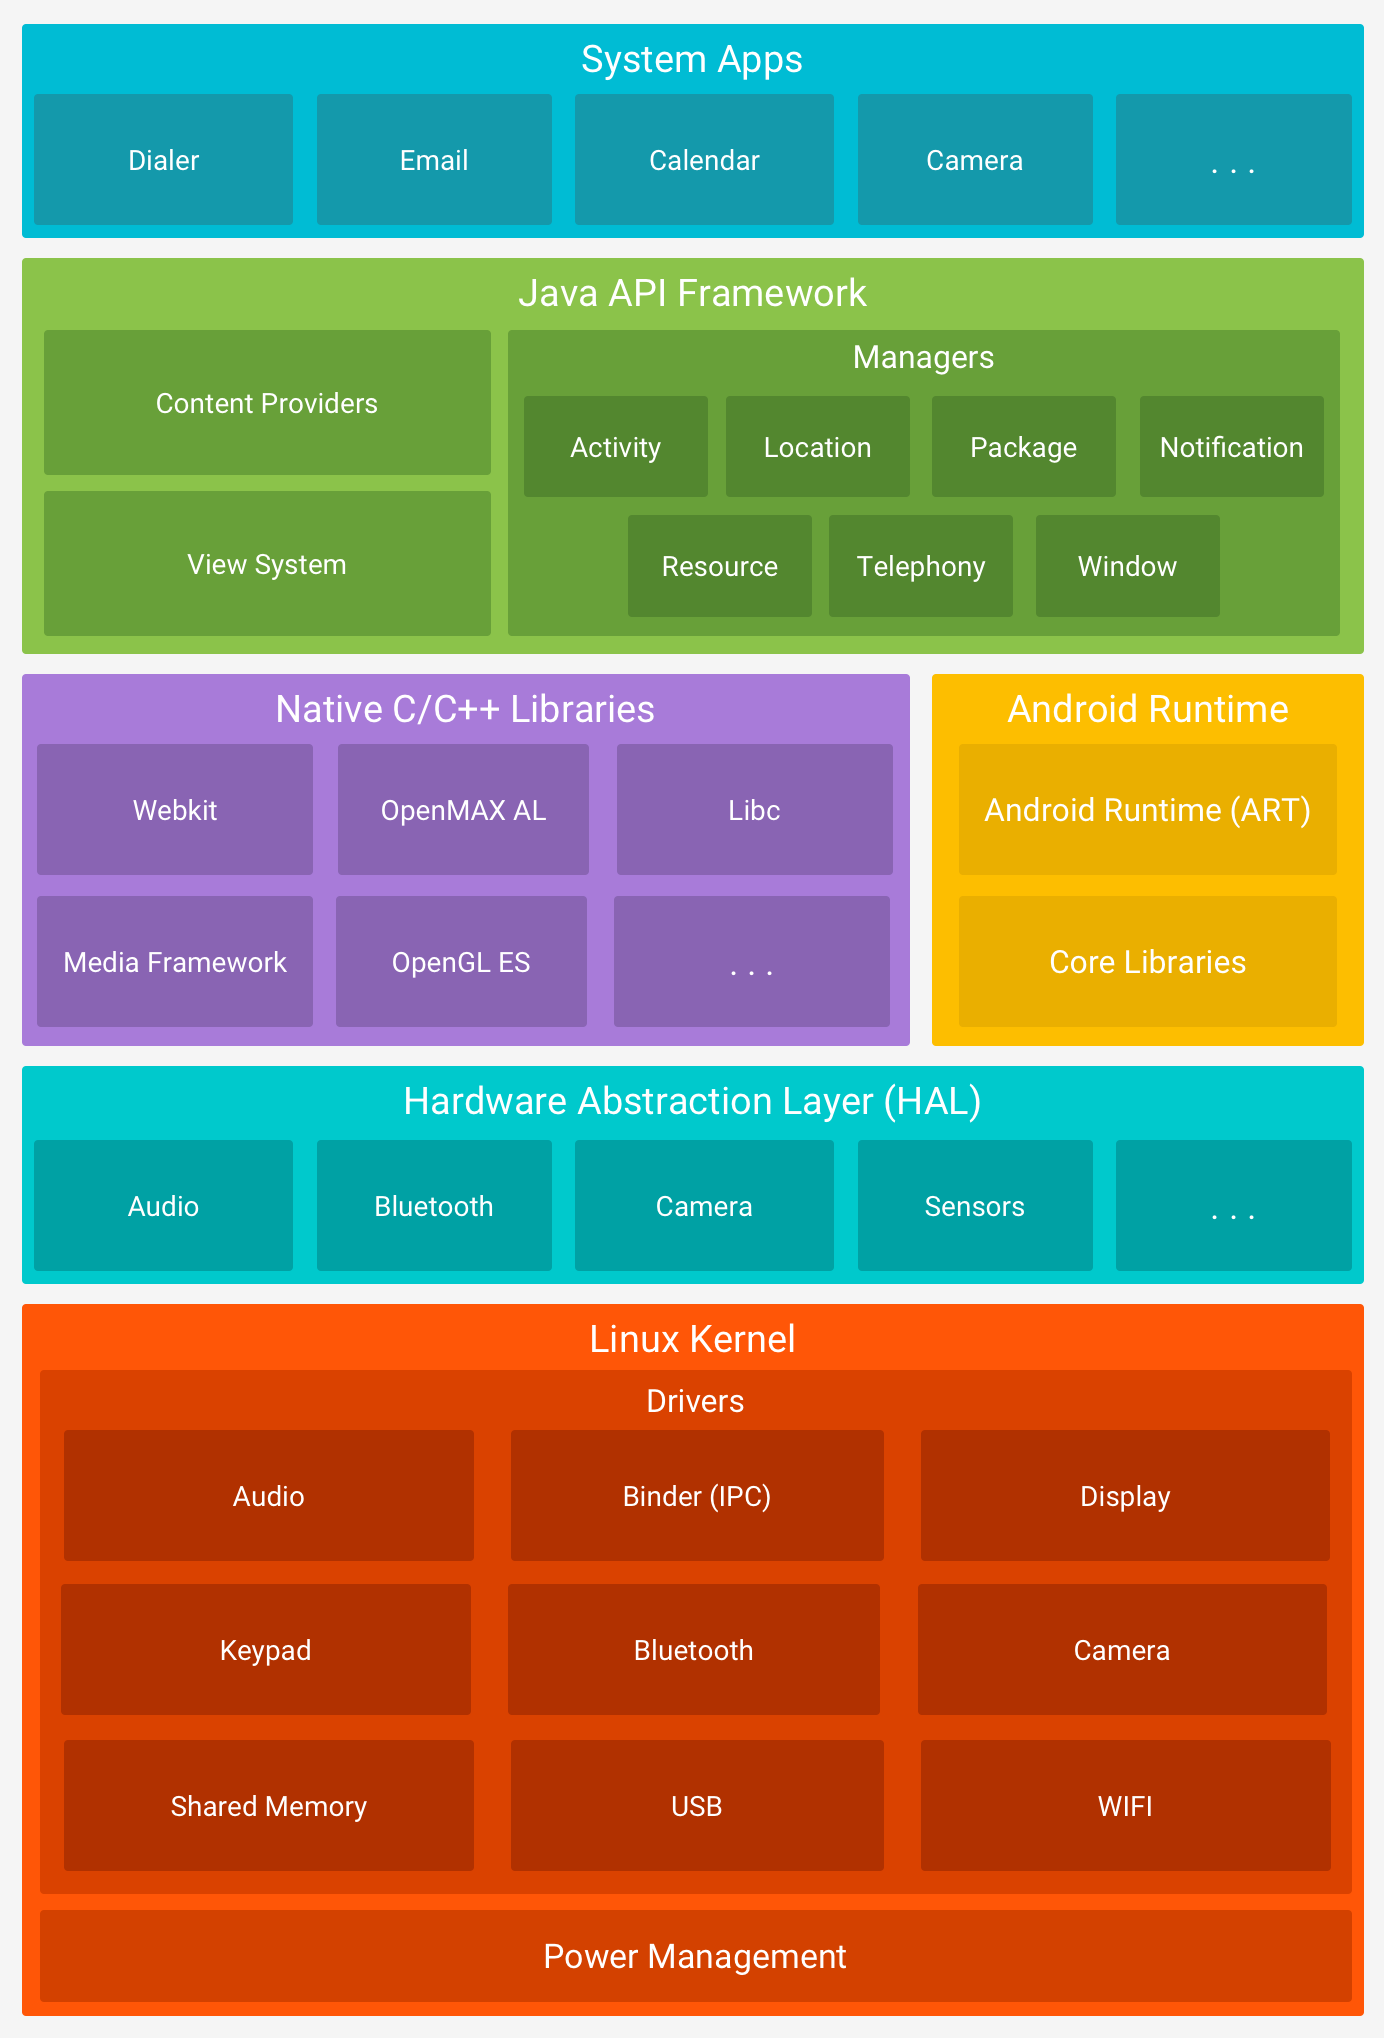
\includegraphics[width=0.5\textwidth]{images/androidstack.png}
	\centering
	\caption[Android stack]{Android is based on the \textit{Linux} kernel. Above, a hardware abstraction layer for the sensors, camera, etc., the \textit{Android} runtime with its core libraries and some native \textit{C++} libraries such as \textit{OpenGL} for the graphics are implemented. Based on this, the well known \textit{Java} API framework which provides the libraries accessible for developers helps for programming software in the high level language \textit{Java}.\footnotemark}
	\label{fig:androidstack}
\end{figure} 

\footnotetext{Image taken from: \url{https://developer.android.com/guide/platform/images/android-stack_2x.png} (24.07.2017)}